\documentclass{article}

\usepackage{amsmath}
\usepackage{graphicx}
\usepackage{titlesec}
\usepackage{lipsum}
\usepackage{url}
\usepackage{float}
\usepackage{fullpage}
\setkeys{Gin}{width=0.50\textwidth}

\titleformat{\section}
  {\normalfont\scshape}{\thesection}{1em}{}

\title{Report 3}
\author{Vanessa Machuca and Luis Espino}

\usepackage{Sweave}
\begin{document}
\Sconcordance{concordance:Report_3.tex:Report_3.Rnw:%
1 17 1 1 0 14 1 1 15 1 8 3 1 1 2 5 0 1 2 2 4 4 1 1 5 3 1 1 10 1 7 2 1 1 %
8 1 1 1 4 1 91 1 1 1 2 1 0 1 1 33 0 1 2 1 1 1 18 2 1 1 2 1 0 1 1 33 0 1 %
2 3 1 1 59 1 2 5 0 1 2 1 1 1 2 1 0 1 1 3 0 1 2 3 1 1 5 5 1 1 6 2 1 1 3 %
17 0 1 2 2 1 1 2 32 0 1 2 5 1 1 5 6 1 1 3 2 0 2 1 3 0 1 2 2 1 1 2 10 0 %
1 2 7 1}

\maketitle

\section{INTRODUCTION}

The data we are working with looks at student achievement in Portuguese course at two secondary education Portuguese schools. We found the data through the UCI Machine Learning Repository. The observational units for the dataset are students. The dataset includes demographic variables like student’s school name (binary), sex (binary), age (numeric), and whether the student lives in an urban or rural area. 

It also includes variables that relate to family, including family size, parents cohabitation status (living apart or together), mother and father's education (ordinal), mother and father’s job ('teacher', 'health' care related, civil 'services' (e.g. administrative or police), 'at$\_$home' or 'other'), student’s guardian (mother, father or other), and quality of family relations ($1$ being very bad to $5$ being excellent). 

School-related variables include home to school travel time (ordinal), weekly study time (ordinal), and number of past class failures (1-3 if $n<3$, 4 otherwise). For each of two courses, students were given a graded after the first and second period as well as a final grade.  
Academic routine, habits and performance were also measured. These variables included travel time from home to school (nominal), weekly study time (nominal), number of past class failures (nominal), reason to choose school (categorical), and number of absences (numeric). Additionally, educational resources were assessed through binary measurements of extra educational support, family educational support, extra paid classes within the course subject, extracurricular activities, attended nursery school, college aspiration, and home internet access.

Finally, nominal variables that measured more personal aspect of life included frequency of outings with friends, workday alcohol consumption, weekend alcohol consumption, current health status, and being in a romantic relationship (binary). 



\section{DATA EXPLORATION}
Let's begin by looking at the pairs plots for four continuous variables- final grade, age, number of absences, and studytime. 

\begin{Schunk}
\begin{Sinput}
> pairs(G3~ age + absences + studytime_num, data = student_por_n)
\end{Sinput}
\end{Schunk}
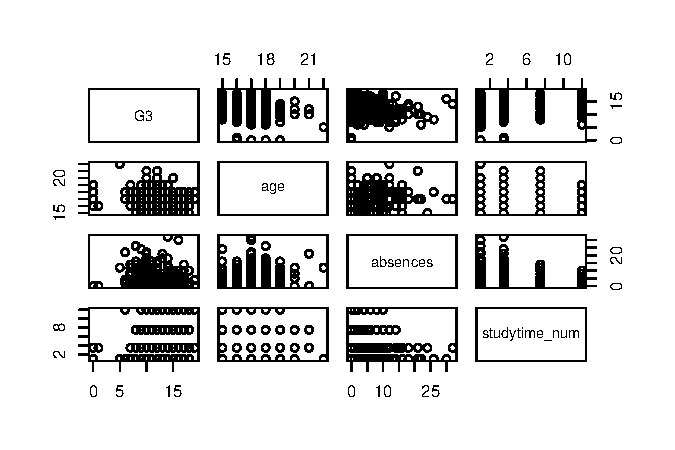
\includegraphics{Report_3-003}



From the pairs plot, we see that there is some linear correlation between absences and weekly study time. The correlation coefficient is -0.11, so the correlation is not very strong. We can also see some correlation between weekly time spent studying and final grade, G3. The correlation coefficient is a little higher, at 0.24, yet still relatively weak. Thus, we will not worry too much about multicolinearity.

From the pairs plot, we also observe that the bulk of the observations in the age variable are between ages 15 and 19. Thus, we group all the students who are older than 19 years old together. Additionally, we can also see that there are some outliers within the absences variable. We filter students who have had more than 30 absences. By constricting our data in this way, we also constrict the population we can generalize to. 


Notice also that four ordinal variables have a very small number of observations for some of their categories. Number of failures has only 13 observations for 2 and 3 failures each. Thus, we lump these categories together. Quality of family relationships, numbered 1-5, with 1 being very bad and 5 being excellent, has only 21 and 29 observations for categories 1 and 2. Thus, we will lump categories 1 and 2 together. We will also lump categories 4 and 5 to balance the range of values that variable categories cover for this variable. Thus, category 1 now represents "bad family relationships," category 2 represents "okay family relationships," and category 3 represents "good family relationships." We do the same for the nominal variables workday alcohol consumption, Dalc. For home to school travel time, the categories are as follows: 1 - <15 min., 2 - 15 to 30 min., 3 - 30 min. to 1 hour, or 4 - >1 hour. Category 4 has only 16 observations. Thus, we combine it with category 3 so that category 3 now represents "more than ">30 minutes of travel time."




\section{MODEL BUILDING}
We use backward and forward selection to determine what variables to include in our model. To do this, we generate training and test sets and build the models on the training set, at $\alpha = 0.05$. 




%Backward Selection Model at 
\begin{Schunk}
\begin{Sinput}
> bkwdselec <- lm(G3~school + sex + Mjob + failures + higher + famrel + Dalc + health, data=col.trn)
> summary(bkwdselec)
\end{Sinput}
\begin{Soutput}
Call:
lm(formula = G3 ~ school + sex + Mjob + failures + higher + famrel + 
    Dalc + health, data = col.trn)

Residuals:
     Min       1Q   Median       3Q      Max 
-11.3921  -1.5330   0.1508   1.4764   6.7290 

Coefficients:
             Estimate Std. Error t value Pr(>|t|)    
(Intercept)  11.69661    0.87636  13.347  < 2e-16 ***
schoolMS     -1.21907    0.29848  -4.084 5.38e-05 ***
sexM         -1.05286    0.28460  -3.699 0.000247 ***
Mjobhealth    0.95806    0.60334   1.588 0.113122    
Mjobother     0.14637    0.37125   0.394 0.693601    
Mjobservices  0.77540    0.44778   1.732 0.084132 .  
Mjobteacher   1.57507    0.51093   3.083 0.002198 ** 
failures     -2.27523    0.30600  -7.435 6.77e-13 ***
higheryes     1.33211    0.46722   2.851 0.004590 ** 
famrel        0.54980    0.21900   2.510 0.012464 *  
Dalc         -0.59288    0.28346  -2.092 0.037129 *  
health       -0.28378    0.09483  -2.993 0.002944 ** 
---
Signif. codes:  0 ‘***’ 0.001 ‘**’ 0.01 ‘*’ 0.05 ‘.’ 0.1 ‘ ’ 1

Residual standard error: 2.686 on 387 degrees of freedom
Multiple R-squared:  0.3507,	Adjusted R-squared:  0.3322 
F-statistic:    19 on 11 and 387 DF,  p-value: < 2.2e-16
\end{Soutput}
\end{Schunk}

%Forwards Selection

%Forwards Selection Model with $\alpha$-to-enter of 0.05. 

\begin{Schunk}
\begin{Sinput}
> fwdselec <- lm(G3~failures+school+sex+higher+health+famrel+Mjob+Dalc, data=col.trn)
> summary(fwdselec)
\end{Sinput}
\begin{Soutput}
Call:
lm(formula = G3 ~ failures + school + sex + higher + health + 
    famrel + Mjob + Dalc, data = col.trn)

Residuals:
     Min       1Q   Median       3Q      Max 
-11.3921  -1.5330   0.1508   1.4764   6.7290 

Coefficients:
             Estimate Std. Error t value Pr(>|t|)    
(Intercept)  11.69661    0.87636  13.347  < 2e-16 ***
failures     -2.27523    0.30600  -7.435 6.77e-13 ***
schoolMS     -1.21907    0.29848  -4.084 5.38e-05 ***
sexM         -1.05286    0.28460  -3.699 0.000247 ***
higheryes     1.33211    0.46722   2.851 0.004590 ** 
health       -0.28378    0.09483  -2.993 0.002944 ** 
famrel        0.54980    0.21900   2.510 0.012464 *  
Mjobhealth    0.95806    0.60334   1.588 0.113122    
Mjobother     0.14637    0.37125   0.394 0.693601    
Mjobservices  0.77540    0.44778   1.732 0.084132 .  
Mjobteacher   1.57507    0.51093   3.083 0.002198 ** 
Dalc         -0.59288    0.28346  -2.092 0.037129 *  
---
Signif. codes:  0 ‘***’ 0.001 ‘**’ 0.01 ‘*’ 0.05 ‘.’ 0.1 ‘ ’ 1

Residual standard error: 2.686 on 387 degrees of freedom
Multiple R-squared:  0.3507,	Adjusted R-squared:  0.3322 
F-statistic:    19 on 11 and 387 DF,  p-value: < 2.2e-16
\end{Soutput}
\end{Schunk}

It turns out that both models utlize the same values! They are the same. Now we will investigate possible interaction terms to add to our forward selection model.

\textbf{Interaction}

\begin{Schunk}
\begin{Sinput}
> ggplot(data = col.trn, aes(x= Dalc, y=G3, color=higher)) + geom_smooth(method='lm',formula=y~x)
\end{Sinput}
\end{Schunk}
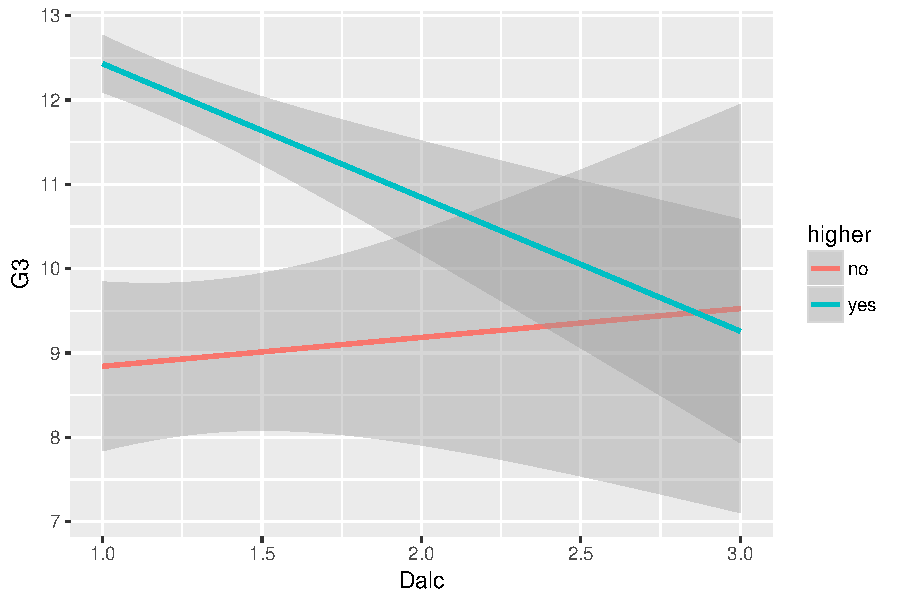
\includegraphics{Report_3-016}


\begin{Schunk}
\begin{Sinput}
> inter <- lm(G3 ~ higher*Dalc,data = col.trn)
> summary(inter)
\end{Sinput}
\end{Schunk}

We looked at all the possible interaction terms and the only significant one at the 0.05 value was between workday alcohol consumption, Dalc, and whether or not a student wants to go to higher education. The interaction does not make sense within the context of this problem, so we will omit it from the model. 

Additionally, based on the VIF values for our model, we do not have a multicolinearity problem. 


\section{MODEL SELECTION}

Now we will compare our model with a nested model with two fewer variables.
%Nested F-Tests

"Dalc" and "famrel" are the least significant of those included in our model. Thus, we will omit them to generate a nested model with two fewer variables than the original. We will now test the hypothesis that both "Dalc" and "famrel" are not needed in the model - $H_{0}=\beta_{Dalc}=\beta_{famrel}=0$ - using a nested F-test. 

\begin{Schunk}
\begin{Sinput}
> #compare each with anova
> anova(fwdselec, fwdselec_reduced)
\end{Sinput}
\begin{Soutput}
Analysis of Variance Table

Model 1: G3 ~ failures + school + sex + higher + health + famrel + Mjob + 
    Dalc
Model 2: G3 ~ failures + school + sex + higher + health + Mjob
  Res.Df    RSS Df Sum of Sq      F   Pr(>F)   
1    387 2791.9                                
2    389 2869.0 -2   -77.103 5.3439 0.005136 **
---
Signif. codes:  0 ‘***’ 0.001 ‘**’ 0.01 ‘*’ 0.05 ‘.’ 0.1 ‘ ’ 1
\end{Soutput}
\end{Schunk}

We get a p-value of 0.0087, indicating, at the $\alpha=0.05$ level, that we can reject the null hypothesis. Indeed, "Dalc" and/or "famrel" are needed in the model. Let's take a quick look at the significance of the variables in the reduced model.

\begin{Schunk}
\begin{Sinput}
> summary(fwdselec_reduced)
\end{Sinput}
\begin{Soutput}
Call:
lm(formula = G3 ~ failures + school + sex + higher + health + 
    Mjob, data = col.trn)

Residuals:
    Min      1Q  Median      3Q     Max 
-11.395  -1.493  -0.023   1.701   6.605 

Coefficients:
             Estimate Std. Error t value Pr(>|t|)    
(Intercept)   12.3425     0.6345  19.452  < 2e-16 ***
failures      -2.4385     0.3053  -7.988 1.56e-14 ***
schoolMS      -1.2776     0.3008  -4.248 2.71e-05 ***
sexM          -1.1187     0.2822  -3.964 8.77e-05 ***
higheryes      1.4386     0.4713   3.053  0.00242 ** 
health        -0.2527     0.0951  -2.657  0.00820 ** 
Mjobhealth     0.9377     0.6083   1.541  0.12401    
Mjobother      0.1551     0.3754   0.413  0.67968    
Mjobservices   0.7528     0.4527   1.663  0.09709 .  
Mjobteacher    1.5620     0.5164   3.024  0.00266 ** 
---
Signif. codes:  0 ‘***’ 0.001 ‘**’ 0.01 ‘*’ 0.05 ‘.’ 0.1 ‘ ’ 1

Residual standard error: 2.716 on 389 degrees of freedom
Multiple R-squared:  0.3328,	Adjusted R-squared:  0.3173 
F-statistic: 21.56 on 9 and 389 DF,  p-value: < 2.2e-16
\end{Soutput}
\end{Schunk}

Interesting - "higheryes" has become significant at the 0.001 level, whereas it was not in the full model. This would indicate collinearity. That said, its significance only very slightly increased. Let's continue working with the full model.


\section{MODEL INTERPRETATION AND FIT}


Our final model is:
$$E[Y]=12.27-1.88X_{failures}-1.25X_{schoolMS}-0.98X_{sexM}+1.42X_{higheryes}-0.27X_{health}+028X_{famrel}$$
$$+0.82X_{Mjobhealth}+0.09X_{Mjobother}+0.77X_{Mjobservices}+1.58X_{Mjobteacher}-0.36X_{Dalc} $$

All $\beta$ coefficients but for those attached to Mjobother,Mjobservices, and Mjobhealth are significant at the 0.05 level. The $\beta$ coefficients for terms failures, schoolMS, sexM, Dalc, and health are negative, where schoolMS and sexM are binary while failures and health are categorical. This relates students being male, drinking more during the day, having more past failures, having better health and attending Mousinho da Silviera with lower scores. Some of these make intuitive sense, while others, particularly regarding health, do not. On the other hand, students wishing to pursue higher education, having strong family relations, and having a mother who works in health, services, teaching, or other is associated with higher scores. These make a bit more sense. 
Let's calculate the CIs for a mean predicted value and a future predicted value for students who go to Gabriel Pereira, mothers work in services, have had 1 failure, are female, have moderately strong family relations, and who drink a moderate ammount during the day, are in okay health and want to pursure higher education.
\begin{Schunk}
\begin{Sinput}
> newset1 <- data.frame(school="GP",Mjob="services",sex="F",famrel=2,Dalc=2,
+                       health=3,failures=1,higher="yes")
> predict.lm(fwdselec,newdata=newset1,interval = "confidence",leve=.95)
> predict.lm(fwdselec,newdata=newset1,interval = "prediction",leve=.95)
\end{Sinput}
\end{Schunk}

We are $95\%$ confident that the true average final grade for these students  is between 9.583384 and 11.59941, and that an individual's future final score is between 5.215242 and 15.96755. 

\begin{Schunk}
\begin{Sinput}
> glance(fwdselec)
\end{Sinput}
\begin{Soutput}
  r.squared adj.r.squared    sigma statistic      p.value df    logLik     AIC
1  0.350688     0.3322321 2.685914   19.0014 1.903073e-30 12 -954.2848 1934.57
       BIC deviance df.residual
1 1986.426 2791.869         387
\end{Soutput}
\end{Schunk}
The $R^2$ for this model is 0.350688 and $R_{adj.}^2$ is 0.3322321. We can go through calculate the $R^2$ for each variable as well. This will tell us how much variation in final grade is explained by adding in each term, assuming all others remain in the model.


\section{SUMMARY}
In summary, we developed a model of 6 variables to predict the final grades for students in Portuguese and math classes at two Portuguese secondary schools. We used forward and backward selection to determine a set of six variables to include in the model. We investigated possible interaction terms as well as a four variable nested model, but decided to stick with the full model. A model such as this might be useful for exploring the affects on factors such as parent occupation and past failure on future academic outcomes. This model could be improved by investigating other possible nested models and carrying out analysis on the sort of effects individual variables might have on variability. 


\end{document}
